\subsection{Low Carbon Future}
\begin{frame}
  \frametitle{Low Carbon Future}
  \begin{figure}
    \centering
    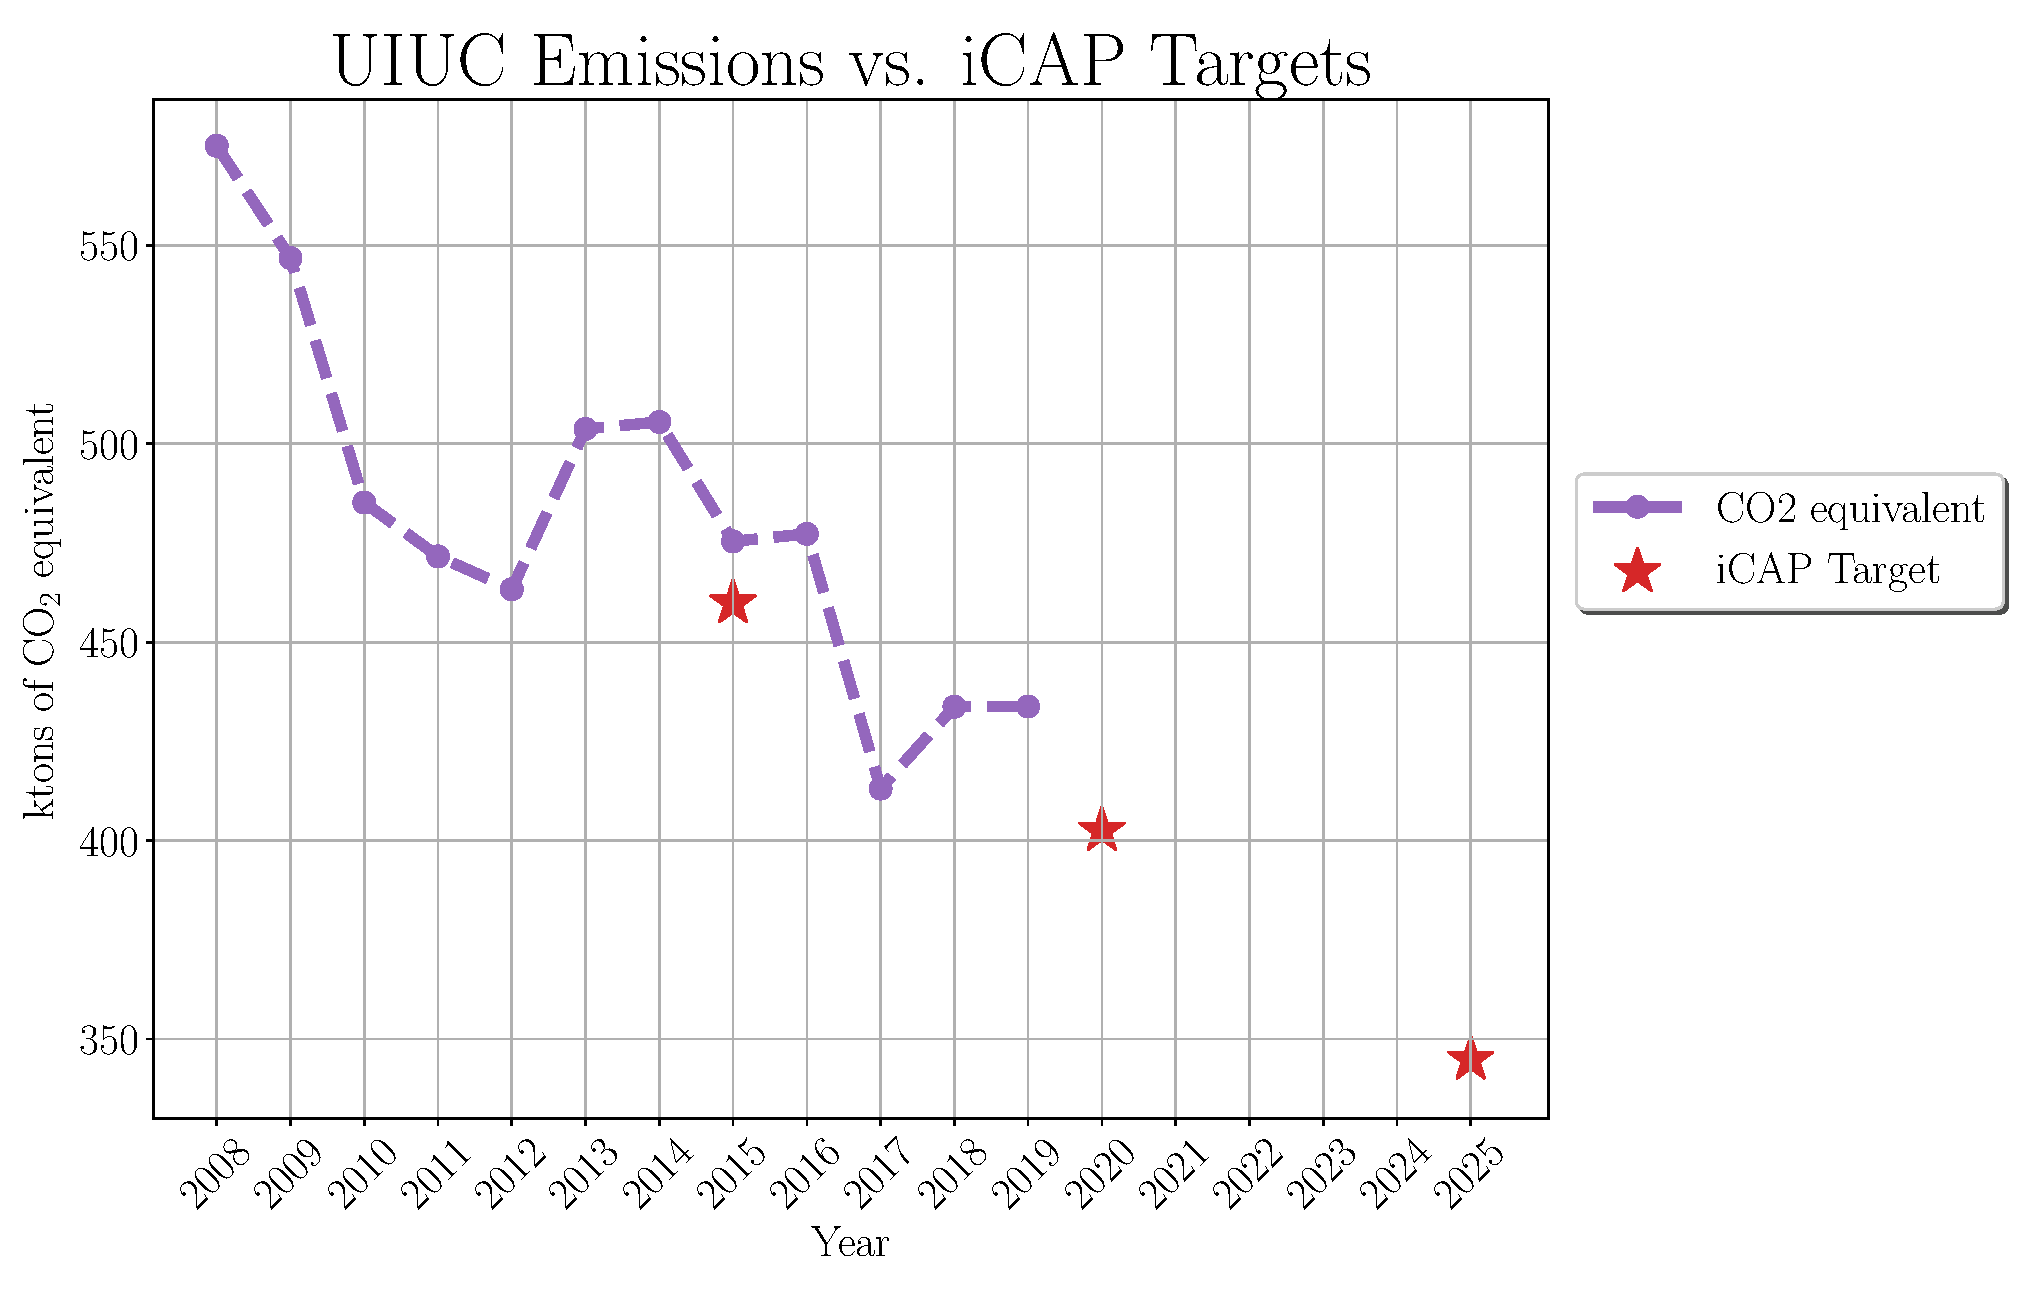
\includegraphics[width=0.8\textwidth]{icap_goals.eps}
    \caption{Carbon emissions goals for the University of Illinois at Urbana-Champaign, outlined in the Illinois Climate Action Plan (iCAP) \cite{isee_illinois_2015}.}
    \label{fig:icapgoals}
  \end{figure}
\end{frame}

\subsection{Rising Renewable Penetration}
\begin{frame}
  \frametitle{Rising Renewable Penetration}
  \begin{figure}
    \centering
    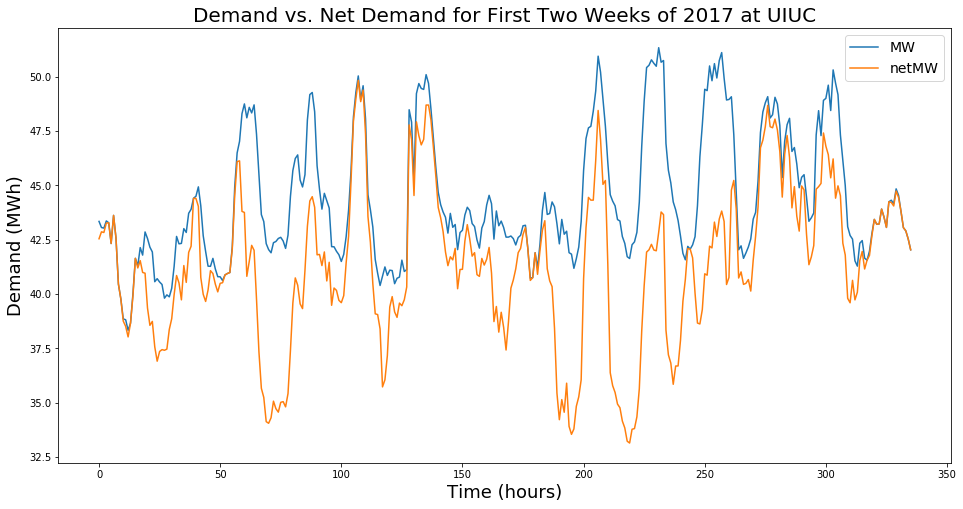
\includegraphics[width=\textwidth]{renewable_variability.png}
    \caption{Comparison between total demand and demand accounting for renewable energy. ``netMW'' is the total demand minus wind and solar \cite{alsoenergy_university_2019, uiuc_illini_2019}. }
    \label{fig:variability}
  \end{figure}
\end{frame}

\subsection{Dilemma for Nuclear Power}
\begin{frame}
  \frametitle{Dilemma for Nuclear Power}
  \begin{figure}
    \centering
    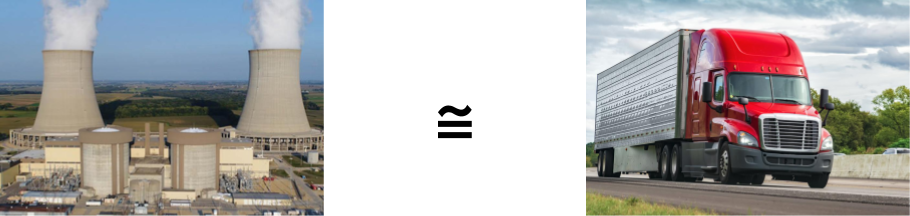
\includegraphics[width=\textwidth]{nukeistruck.png}
    \caption{Traditional nuclear plants are like semi-trucks. They carry a lot of freight but can't turn very fast. Left: Byron Nuclear Station}
    \label{fig:semitruck}
  \end{figure}
\end{frame}
